\documentclass{article}
\usepackage{graphicx}% Required for inserting images
\usepackage{lindrew}
\usepackage[shortlabels]{enumitem}
\usepackage{pdfpages}
\usepackage{enumerate}
\usepackage{algorithm}
\usepackage{algpseudocode}
\usepackage{matlab-prettifier}
\usepackage{pythonhighlight}

\title{CS 156a Problem Set 6}
\author{Amitesh Anand Pandey}
\date{October 2024}

\begin{document}
\maketitle
\section*{Linear Regression Error}
\subsection*{Problem 1}
 Since $\mathcal{H}' \subset \mathcal{H}$, in general, it will fail to explain as much of $f$ as $\mathcal{H}$ and the deterministic noise will increase, option $\textbf{[b]}$.
 \section*{Regularization with Weight Decay}
 \subsection*{Problem 2}
 From running the code in the appendix, we get the closest error as $(0.03, 0.08)$, so $\textbf{[a]}$ is the correct option.
 \subsection*{Problem 3}
 From running the code in the appendix, we get the closest error for $k = -3$ as $(0.03, 0.08)$ again, so $\textbf{[d]}$ is correct. 
 \subsection*{Problem 4}
 From running the code in the appendix, we get the error as $(0.37, 0.44)$ for $k = 3$, so the closest option is $(0.4, 0.4)$, so the correct option is $\textbf{[e]}$.
 \subsection*{Problem 5}
 From running the code in the appendix, we find that $k = -1$ minimizes out of sample error rate of classification so the correct option is $\textbf{[d]}$.
 \subsection*{Problem 6}
 From varying $k$ between $[-50, 50)\cap\mathbb{Z}$, we find that the smallest out of sample error is $0.056$, closest to $0.06$, so $\textbf{[b]}$.
\newpage
\section*{Regularization with Polynomials}
\subsection*{Problem 7}
Let's look at $\mathcal{H}(10, 0, 3)$ first, by definition we have
\begin{align*}
\mathcal{H}(10,0,3)&=\left\{h \mid h(x)=\sum_{q=0}^{10} w_q L_q(x); w_q=0 \text { for } q \geq 3\right\}\\
&=\left\{h \mid h(x)=\sum_{q=0}^2 w_q L_q(x)\right\} = \mathcal{H}_2
\end{align*}
\begin{equation*}
    \mathcal{H}(10, 0, 4) = \mathcal{H}_3
\end{equation*}
Now we make the observation that necessarily for $\forall i, j \in\mathbb{N}$, if $i < j$, then $\mathcal{H}_{i} \subset \mathcal{H}_{j}$, this is a logical conclusion from the definitions in the question. Set theoretically, we also know $\mathcal{H}_{i} \subset \mathcal{H}_{j} \implies \mathcal{H}_{i} \cap \mathcal{H}_{j} = \mathcal{H}_{i}$. This brings us to the fact that $\mathcal{H}(10, 0, 3) \cap \mathcal{H}(10, 0, 4) = \mathcal{H}_{2} \cap \mathcal{H}_{3}$ given $\mathcal{H}_{2} \subset \mathcal{H}_{3}$ this implies directly that $\mathcal{H}_{2} \cap \mathcal{H}_{3} = \mathcal{H}_2$. So the correct option then is option $\textbf{[c]}$.
\section*{Neural Networks}
\subsection*{Problem 8}
First, for the forward pass, operations of the form $w_{ij}^{(l)}x_{i}^{(l-1)}$, we  have 2 layers, for the first layer, there are 5 inputs causing 2 operations each for this results in 10 operations. In the second layer, we effectively have 3 inputs sending 1 signal each, this results in 3 operations, so the forward pass has 13 operations in total. In the backward pass, we have the final layer sending 1 signal each to three ``inputs" of the second layer, resulting in 3 operations. Then two non trivial nodes of the second layer each send 5 signals (one to each node of the first layer). This results in 13 operations. Each of these bring about a corresponding update to the weight vector, which means there are 13 total updates to the weight vector systematically at each of these steps. Finally, once back propagation has wrapped up, there is an ultimate update to the weight vector once again causing 5 operations, so the total operations taken is 44, closest to 45, which is option  $\textbf{[d]}$. 
\subsection*{Problem 9}
The total weights are reduced greatly when there is only one weight to pass over from one unit of the hidden layer to another. We are forced by the question to have 10 units sending a signal each to a 1-node first unit, causing 10 weights. Now we have 36 units, which require $\left\lceil\frac{36 - 1}{2}\right\rceil$ weights to reach the final layer. This gets us to 18 weights. For each of these units, there is also the trivial node causing 1 weight for each unit traversal, causing 18 more units. Thus we have $10 + 18 + 18 = 46$ weights, equal to option $\textbf{[a]}$. 
\subsection*{Problem 10}
This problem does appear tedious calculatively, and I have run out of time to code this. Because of the nature of the question, I am \textbf{guessing} the largest possible $\textbf{[e]}$ is correct.

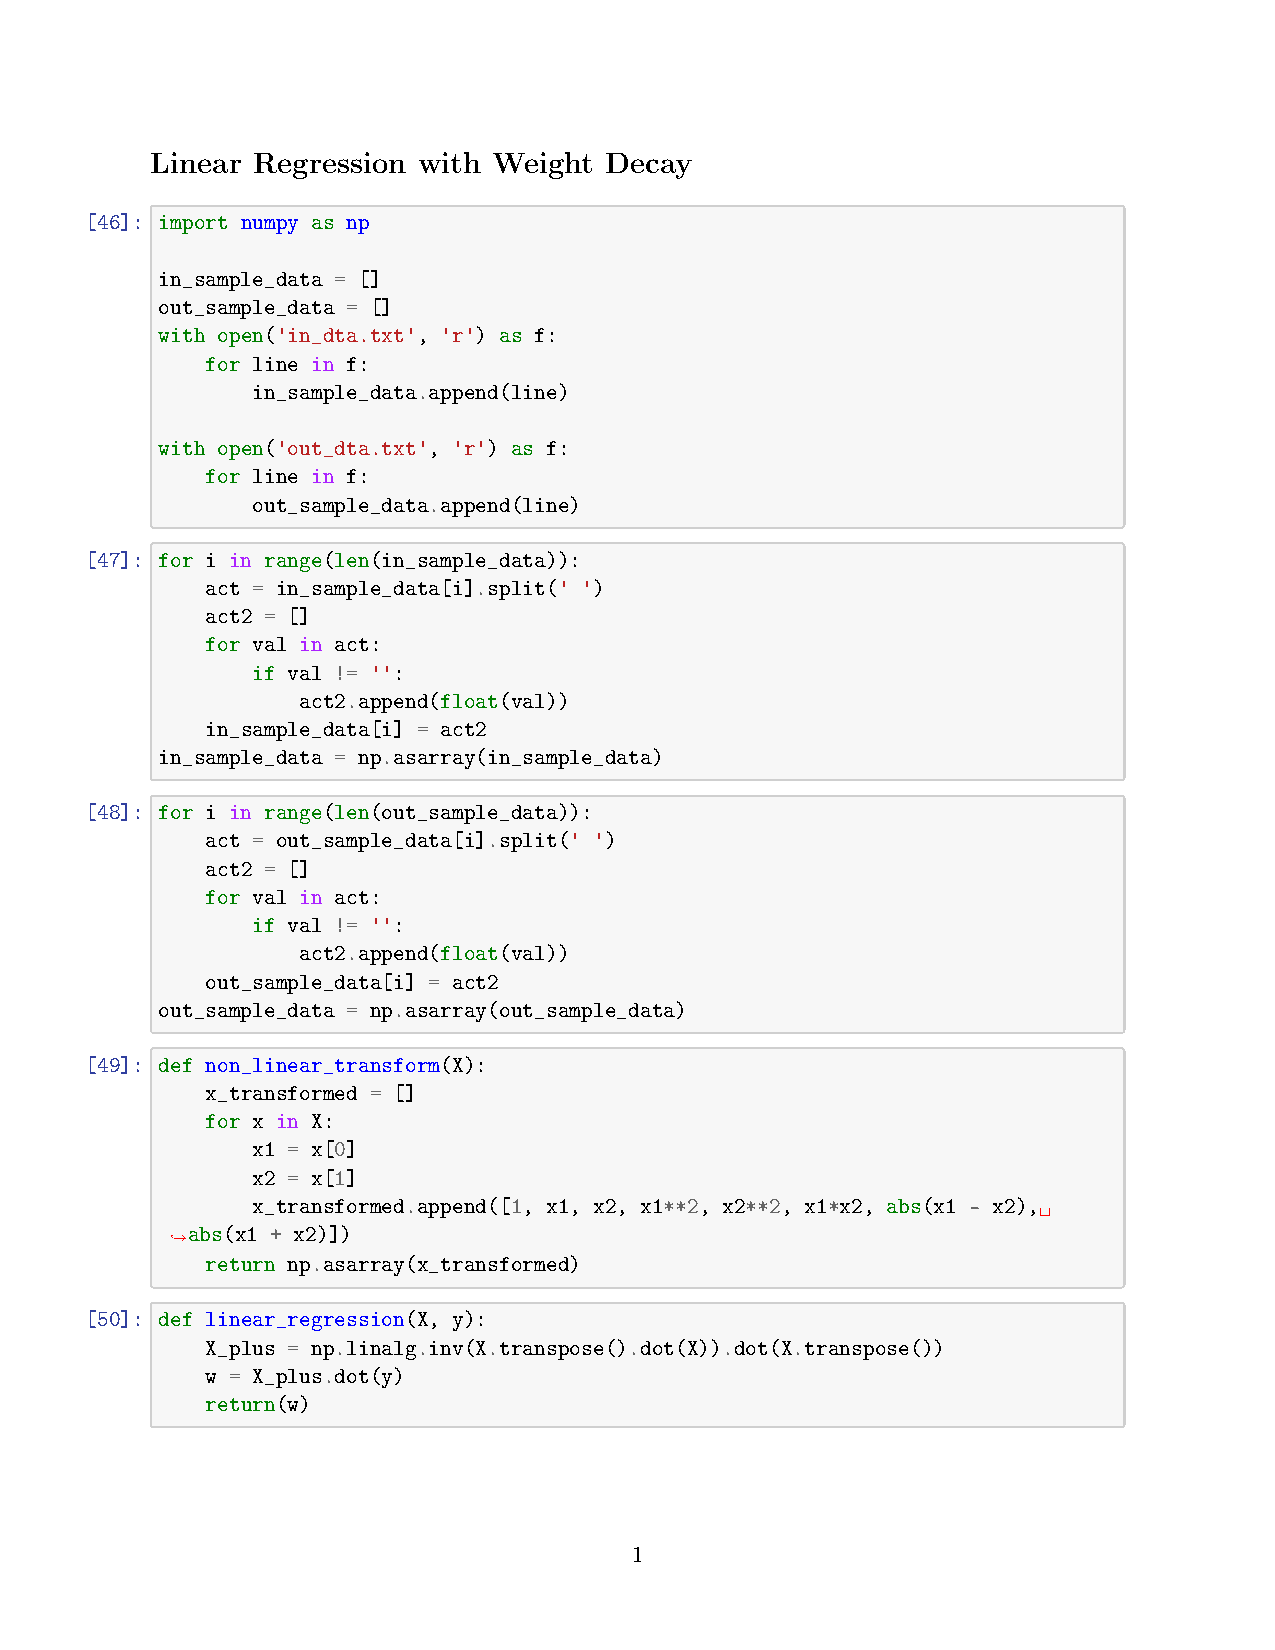
\includepdf[pages=-]{Code_for_HW6.pdf}
\end{document}
